\subsection{Animatie met timers}
<<<<<<< Updated upstream

Een animatie wordt vloeiend bevonden als er geen frame ontbreekt tijdens het afspelen. Hoe meer frames er per seconde afgebeeld kunnen worden, hoe vloeiender de animatie oogt. Het gemiddelde consumer-device heeft een refresh rate van 60Hz wat overeenstemt met 60 frames per seconde (fps). Om een animatie zo vloeiend mogelijk te laten afspelen, wordt er dus over het algemeen gemikt naar een afspeelsnelheid van 60fps.
=======
Een animatie wordt smooth bevonden als er geen frame ontbreekt tijdens het afspelen. Hoe meer frames er per seconde afgebeeld kunnen worden, hoe smoother de animatie oogt. Het gemiddelde consumer-device heeft een refresh rate van 60Hz wat overeenstemt met 60 frames per seconde (fps). Om een animatie zo smooth mogelijk te laten afspelen, wordt er dus over het algemeen gemikt naar een afspeelsnelheid van 60fps.
>>>>>>> Stashed changes

Om elke seconde 60 frames af te beelden moeten de frames volgens een correct getimed interval de volgende frame afbeelden. In javascript zijn hier twee build-in functies voor beschikbaar, \texttt{setTimeout()} en \texttt{setInterval()}. Op deze manier kan er met een timer om de 16.7ms een nieuwe frame afgebeeld worden om de 60fps playback snelheid te behalen.

\subsection{Problemen met timers}
Bij het gebruik maken van timers wordt er verondersteld van een playback van 60fps omdat de meeste schermen dit hanteren, maar als er een trager scherm gebruikt wordt om deze animatie af te beelden zullen er overtollige frames ingeladen worden niet gerenderd zullen worden door de browser. Een laadtijd van 16.7ms of minder voor elke frame is ook niet gegarandeerd en wordt verder besproken in \ref{performance}.

\paragraph{Drift in timers}Deze timers zouden er voor zorgen dat er elke gerenderde frame door de browser, de juiste frame van de animatie bevat. Dit kan niet aangenomen worden aangezien er altijd een kleine fout zal bestaan op de wachttijd tot de executie van de opgeroepen functie van de timer. Bij het uitvoeren van een test gebaseerd op \cite{testDrift} valt te constateren dat veel populaire browsers de kleine fout niet compenseren en daardoor begint op te tellen en als gevolg de globale timing van de animatie volledig zijn synchronisatie verliest.

\begin{figure} [H]
	\centering
	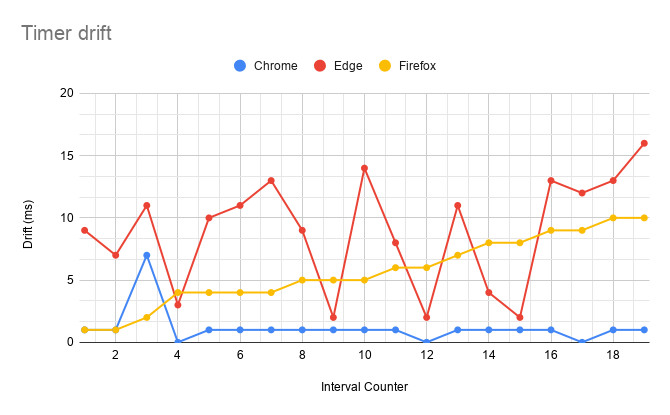
\includegraphics [width=0.7\textwidth] {img/Timer drift.png}
	\caption{Timer drift van verschillende populaire browsers} \label{drift}
\end{figure}

Door het continu opschuiven van frame updates kan er een framedrop voorkomen door redundante stappen van de animatie in te laden tijdens de foute frame waardoor de animatie stappen verliest en haperend ervaren wordt.

\paragraph{Single threaded}
Javascript wordt single-threaded in de browser uitgevoerd. Door deze limitatie kan een taak die getimed staat over x aantal milliseconden pas uitgevoerd worden op de main thread als de event loop op dat moment beschikbaar is om die functie dan uit te voeren. Als er tussen het initialiseren van de timer en het uitvoeren van deze geplande taak een andere taak tussenbeide komt die langere executietijd heeft dan de geplande tijd zal de uitvoering uitgesteld worden tot de event loop terug vrij komt. Ook dit is een deuk in de betrouwbaarheid van timers en kan voor framedrops zorgen als de executie te lang wordt uitgesteld tot voor de nieuwe repaint.

\begin{figure} [H]
	\centering
	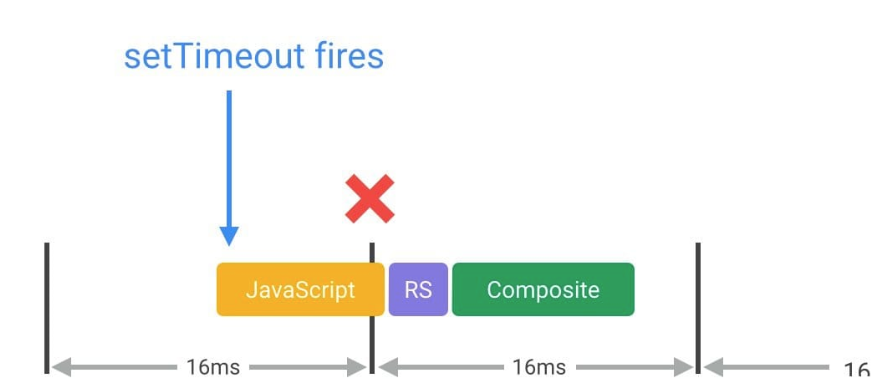
\includegraphics [width=0.6\textwidth] {img/drift-framedrop.png}
	\caption{Framedrop door gebruik van setTimeout. (Afbeelding van Google Web Fundamentals \cite{frameDrop:img})} \label{drift-framedrop}
\end{figure}

\subsection{RequestAnimationFrame}

Een methode die moderne browsers bieden om animaties te updaten met javascript is \texttt{requestAnimationFrame()}. Het wordt in dezelfde context gebruikt als \texttt{setTimeout()}, maar lost enkele cruciale problemen op. Ten eerste moet er geen tijdsinterval meer gespecifieerd worden als parameter, maar synced de browser de executie van deze taak met de refreshrate van de monitor. De opgegeven callback functie wordt door de event loop net voor de repaint van de pagina uitgevoerd. Hierdoor worden enkel frames geüpdatet voor een repaint en zullen er geen redundante taken uitgevoerd worden per frame of framedrops voorkomen. \cite{requestFrameDocs}

\subsection{Performance} \label{performance}
\texttt{requestAnimationFrame()} lost een groot deel van globale timing op, maar garandeert daarom geen vlotte animation playback. We gaan er verder vanuit dat er geen devices een hogere refresh rate dan 60Hz utiliseren en mikken dus op een playback snelheid van 60fps. Als de methode om de frame te updaten langer duurt dan 16.7ms zal de frame niet gedropt worden, maar uitgetrokken. Alle frames worden wel weergegeven, maar niet aan een snelheid van 60fps wat dus ook oogt als een niet vloeiende animatie.



Om een pagina zo responsief mogelijk te houden, moet het aantal reflows geminimaliseerd worden. Er zijn nog verscheidene elementen die de reflow snelheid beïnvloeden zoals de diepte en afhankelijkheden van nodes in de DOM-tree van de webpagina. Aangezien er in dit geval enkel gewerkt wordt met een enkelvoudige animatie op een eenvoudige webpagina gaan we hier niet verder op in.
\cite{improvePerformance}
